\label{sec:Wettbewerbsanalyse}

Um die Bedürfnisse zukünftiger Nutzer zu erfüllen und das Produkt langfristig wettbewerbsfähig zu halten, ist es unerlässlich, kontinuierlich alle relevanten Kundenanforderungen zu ermitteln und zu priorisieren. Zusätzlich ist es wichtig, sich mit Wettbewerbern, ihren Produkten und Strategien auseinanderzusetzen, um die eigenen Marktchancen zu bewerten. Eine Analyse gibt zudem Aufschluss darüber, welche Features bereits als grundlegend erwartet werden und welche Möglichkeiten es gibt, um sich von anderen Anbietern zu differenzieren.


Die Wettbewerbsanalyse wurde in mehreren Schritten durchgeführt:

\begin{itemize}
    \item Ermittlung der Hauptwettbewerber
    \item Erstellung eines Konkurrenzprofils
    \item Darstellung der einzelnen Wettbewerber
    \item Bewertung der strategischen Ausrichtung
    \item Zusammenfassung der Ergebnisse
\end{itemize}

\subsection{Ermittlung der Hauptwettbewerber}

Für die Identifikation der bedeutendsten Mitbewerber ist es wichtig, die Hauptmerkmale und Ziele des eigenen Dienstes zu kennen und mit potenziellen Wettbewerbern abzugleichen. Dabei sollte berücksichtigt werden, dass es in der digitalen Welt nicht immer Wettbewerber gibt, die exakt den gleichen Dienst anbieten oder dieselbe Strategie verfolgen. Dennoch können mittelfristig vollwertige Konkurrenzprodukte entstehen, die zum Zeitpunkt der Analyse nur wenige gemeinsame Parallelen oder Features aufweisen.

Die langfristige Ausrichtung von \acrfull{dht} besteht darin, den lokalen/regionalen Raum und seine sozialen Verflechtungen zu stärken, indem der digitale Austausch zwischen allen Personen und Institutionen gefördert wird, die das örtliche Dasein widerspiegeln. Die Schwerpunkte von \acrshort{dht} sind wie folgt:

\begin{enumerate}
    \item Das Vernetzen von Personen, die gleiche Interessen oder ähnliche Bedürfnisse haben und einen Austausch von Informationen, Waren und Dienstleistungen anstreben oder Unterstützung und Hilfestellung suchen bzw. anbieten.
    \item Die Stärkung lokaler Vereine und Dienstleistungen, damit diese ihre Angebote gezielter darstellen und leichter mit Interessenten in Kontakt treten können.
    \item Die Unterstützung öffentlicher Einrichtungen, um einen einfacheren Zugang zu amtlichen Informationen, Terminen und anderen Ressourcen zu ermöglichen.
\end{enumerate}

Zugleich verpflichtet sich \acrshort{dht} dazu, allen Nutzern einen barrierefreien Zugang zu ermöglichen.

Basierend auf den Zielen von \acrshort{dht} wurden verschiedene Webdienste identifiziert, die sich auf den lokalen Raum und den Austausch, die Vernetzung oder die Zusammenführung von Privatpersonen konzentrieren. Zunächst wurden als etablierte und aktive Vertreter in mindestens einem der genannten Bereiche identifiziert:

\begin{itemize}
    \item Facebook,
    \item Nebenan.de,
    \item Spontacts,
    \item eBay Kleinanzeigen und
    \item Doctolib.
\end{itemize}

Im Folgenden werden beispielhaft nur die Vertreter aus dem Bereich Social Networking näher betrachtet, zu denen Facebook, Nebenan.de und Spontacts zählen.

\subsection{Konkurrenzprofil}

Für eine eingehende Analyse der ermittelten Wettbewerber ist es notwendig, individuelle Konkurrenzprofile für jeden Marktteilnehmer zu erstellen. Diese Gegenüberstellung des eigenen Selbstprofils bietet eine transparente Bewertungsbasis, die wertvolle Erkenntnisse über Stärken, Potenziale und strategische Ziele liefert.

Folgende Punkte werden bei der Konkurrenzanalyse gesondert betrachtet:

\begin{itemize}
    \item Fokus des Dienstes und Zielgruppe
    \item Möglichkeiten der Selbstdarstellung und des Austauschs
    \item Benachrichtigungen über Änderungen und Neuigkeiten
    \item Entdecken von Inhalten
\end{itemize}

\subsection{Kurzdarstellung}

\subsubsection{Facebook}

\acrfull{fb}\footnote{vgl. Facebook 2023 \cite{facebook}} ist ein weltweit bekannter und etablierter Dienst, der es Nutzern ermöglicht, sich mit Menschen aus aller Welt zu vernetzen, in Kontakt zu bleiben und Inhalte aus ihrem Leben mit anderen zu teilen.
Ursprünglich richtete sich der Fokus von \acrshort{fb}  auf Studenten, aber im Laufe der Jahre hat sich die Zielgruppe verbreitert und ist heute sehr heterogen.

\begin{figure}[!htb]
    \centering
    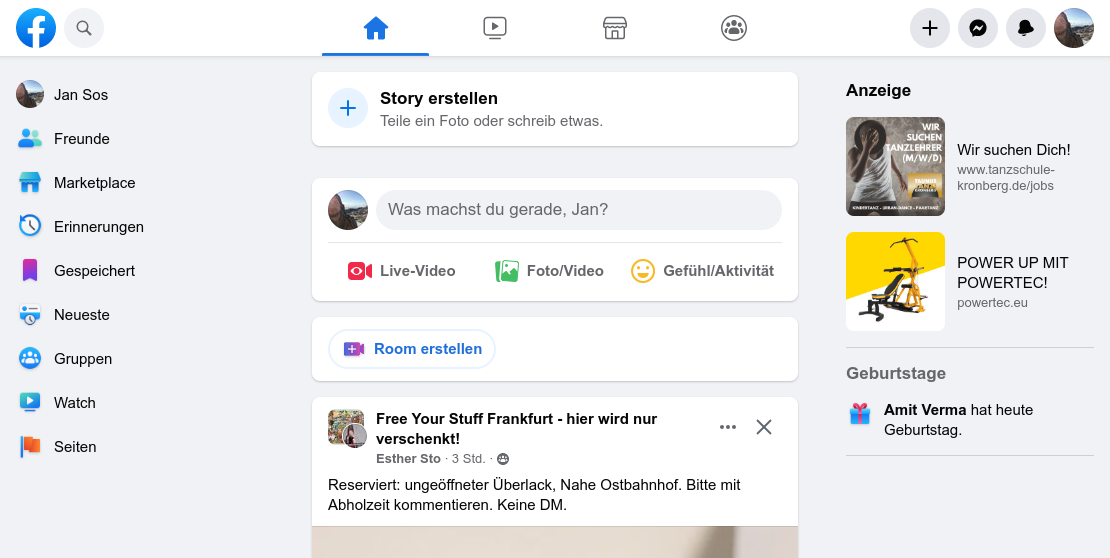
\includegraphics[width=\textwidth]{figures/jan/pic_facebook.png}
    \caption[Startseite von \acrshort{fb}]{Startseite von Startseite von \acrshort{fb}}
    \label{fig:facebook}
\end{figure}

Die Nutzung von \acrshort{fb} ist sehr vielfältig und hängt von den Bedürfnissen des einzelnen Nutzers ab. Neben reinen Darstellungs- und Austauschmöglichkeiten bietet \acrshort{fb} eine breite Palette von Anwendungen an, wie z.B. integrierte Video-, Game- und Datingportale sowie ein eigenes Bezahlsystem. Auf diese speziellen Anwendungen wird im weiteren Verlauf nicht weiter eingegangen.

\paragraph{Selbstdarstellung}

Für die Selbstdarstellung von Organisationen oder Personen bietet \acrshort{fb} ein eigenes Profil an, auf dem Bilder, persönliche Informationen und Vorlieben wie Musik öffentlich dargestellt werden können. Die Sichtbarkeit dieser Inhalte kann individuell angepasst werden. Neben den statischen Informationen enthält das Profil auch eine Pinnwand, auf der ältere und aktuelle Beiträge listenmäßig aufgeführt werden.

\paragraph{Formen des Austausches}

Beiträge ermöglichen den interaktiven Austausch und das Teilen von Momenten. Jeder Nutzer kann sie verfassen und auf seiner eigenen sowie auf fremden Pinnwänden veröffentlichen. Ereignisse wie das Hochladen von neuen Bildern generieren automatisch einen Beitrag, um Bekannte, Follower und andere Personen über Neuigkeiten im Profil zu informieren. Beiträge lassen sich neben einfachem Text auch mit Bildern oder Videos sowie mit Tags (Orte, GPS, Veranstaltungen, Personen, etc.) spezifizieren. Andere Nutzer können Beiträge kommentieren oder bewerten.

\acrshort{fb}-Gruppen ermöglichen den Austausch mit mehreren Personen zu gemeinsamen Themen. Ähnlich wie Profile haben Gruppen einen statischen Teil, in dem Administratoren eine Kurzbeschreibung der Gruppe veröffentlichen. Eine Pinnwand ermöglicht den Mitgliedern die Kommunikation untereinander. Durch das Erstellen von Events können Gruppenmitglieder gemeinsame Treffen oder Aktivitäten planen.\\
Gruppen werden sehr häufig und für verschiedene Themen genutzt. Insbesondere im städtischen Raum dienen sie zum Beispiel dem Verschenken von ungenutzten Dingen, dem Knüpfen neuer Kontakte in einer neuen Stadt oder dem Treffen von Menschen in der Nähe mit ähnlichen Hobbies. Auch der Austausch über diverse Themen in unterschiedlichen Bereichen auf regionaler, nationaler und internationaler Ebene ist weit verbreitet.

Der Austausch materieller Gegenstände findet hauptsächlich auf einem digitalen Marktplatz statt. Die geschalteten Anzeigen enthalten eine Überschrift, eine freie Beschreibung, Bilder, Angaben zum Zustand, zur Preisvorstellung, zum Ort und zum Herausgeber der Anzeige. Der Verfasser muss bei der Erstellung der Anzeige eine vordefinierte Kategorie auswählen, um die Auffindbarkeit zu erleichtern. Neben der direkten Kontaktaufnahme besteht für Interessenten die Möglichkeit, die Anzeige zu merken, mit einem Kontakt zu teilen oder einen Alarm zu erstellen, sobald ähnliche Produkte angeboten werden.

Auf \acrshort{fb} können Kontakte gepflegt werden, indem man sich gegenseitig in eine Freundesliste aufnimmt. Über diese Liste können Inhalte selektiv verteilt werden, so dass sie nur für \textit{Freunde} sichtbar sind. Zusätzlich werden \textit{Freunde} über das Dashboard gezielt informiert, wenn ein \textit{Freund} einen neuen Beitrag erstellt hat.

Für den direkten und privaten Austausch bietet \acrshort{fb} einen Chat an, in dem sowohl 1:1- als auch Gruppenchats möglich sind. Die Kommunikation erfolgt in Echtzeit und die Nachrichten können wie Beiträge Bilder, Links und andere Inhalte enthalten. In 1:1-Gesprächen besteht auch die Möglichkeit, Sprach- und Videoanrufe zu tätigen.

\paragraph{Neuigkeiten}

Um bei der Vielzahl der Beiträge und Reaktionen von Freunden oder Gruppen den Überblick zu behalten, bietet \acrshort{fb} ein Dashboard an, auf dem Neuigkeiten in Form einer endlosen und unsortierten Liste angezeigt werden. Das Dashboard enthält auch kommerzielle Werbung und Beiträge von Gruppen, die der Nutzer noch nicht abonniert hat, aber von Interesse sein könnten.

Neben dem Dashboard gibt es auch eine Notifications-Seite, die einen gezielteren Fokus auf das Wesentliche ermöglicht. Hier werden kurze Benachrichtigungen wie Geburtstage von \textit{Freunden}, bevorstehende Events, neue Beiträge aus abonnierten Gruppen sowie Reaktionen auf eigene oder kommentierte Beiträge angezeigt.

\paragraph{Recherche}

\acrshort{fb} bietet eine Suchfunktion, die es Nutzern ermöglicht, nach Personen, Gruppen und anderen Inhalten zu suchen. Die Suchergebnisse können durch verschiedene Filter wie Art des Inhalts, Verfasser, Gruppen, Zeitraum und mehr genauer spezifiziert werden.

Zusätzlich können Nutzer Beiträge und öffentliche Profile als \textit{Bookmarks} sichern. Die \textit{Bookmarks} können dann auf einer dafür vorgesehenen Seite je nach Typ aufgelistet und verwaltet werden.

\subsubsection{Nebenan.de}

Nebenan.de\footnote{Vgl. nebenan.de 2023 \cite{nebenan}} ist eine Plattform, die im Jahr 2015 gestartet wurde und wie \acrshort{fb} darauf abzielt, Menschen zu vernetzen (Abb. \ref{fig:nebenan}). Der Unterschied zu \acrshort{fb} besteht darin, dass sich Nebenan.de ausschließlich auf die unmittelbare Nachbarschaft des Nutzers konzentriert.

\begin{figure}[!htb]
    \centering
    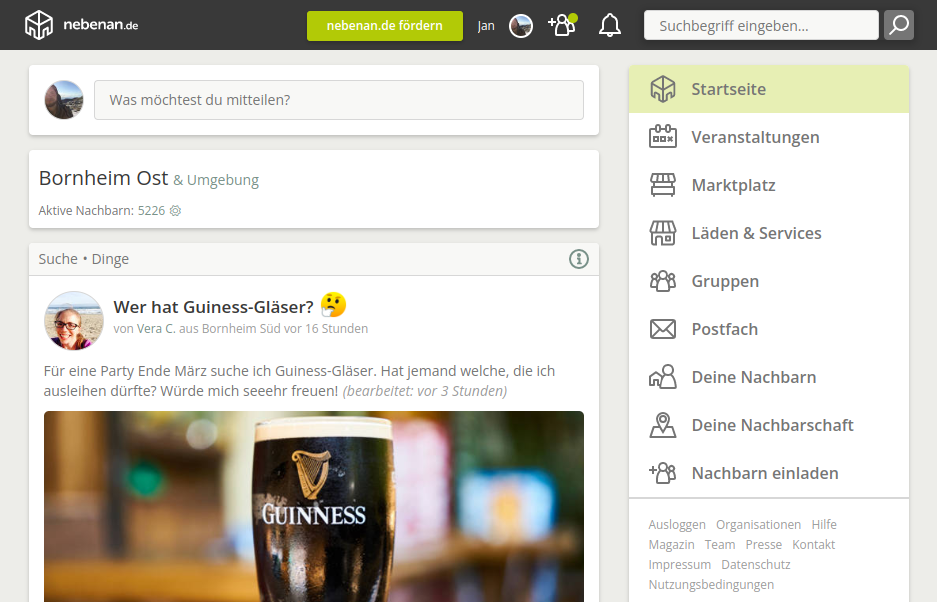
\includegraphics[width=\textwidth]{figures/jan/pic_nebenan.png}
    \caption[Startseite von nebenan.de]{Startseite von nebenan.de}
    \label{fig:nebenan}
\end{figure}

Die Zielgruppe umfasst alle Interessengruppen, die in der Nachbarschaft des Benutzers vertreten sind, wie z.B. Anwohner, Vereine, Firmen und Organisationen. Die Nachbarschaftsgrenze wird vom System anhand der eigenen Adresse des Nutzers definiert und kann nicht individuell angepasst werden.

\paragraph{Selbstdarstellung}

Für die Darstellung existieren auf Nebenan.de zwei Arten von Profilen. Die erste Profilart gilt für Einzelnutzer. Hierbei können sich Anwohner über ein Kurzprofil mit Foto, einem Freitext sowie ihren Interessen und Angeboten vorstellen. Zur Auswahl der Interessen und Angebote gibt es fest definierte Vorschläge, um zu beschreiben, was der Anwohner in die Nachbarschaft einbringen kann. Dazu zählen beispielsweise das \textit{Annehmen von Paketen}, das \textit{Blumengießen}, die \textit{Reparatur von Fahrrädern} oder das \textit{Gesellschaft leisten}. Das Profil zeigt auch die Aktivitäten des Anwohners an, wie beispielsweise beigetretene nebenan-Gruppen und die Anzahl der erhaltenen virtuellen Dankeschöns. \\
Organisationen und Läden/Services, die vor Ort angesiedelt sind und zum alltäglichen Leben in der Nachbarschaft beitragen, nutzen die zweite Profilart. Diese Profile enthalten im Vergleich zu den Anwohnerprofilen deutlich mehr Informationen und müssen beim Anlegen einer Kategorie zugeordnet werden, wie z.B. \textit{Restaurant}, \textit{Reisen}, \textit{Sport}, \textit{Political Party} oder \textit{Nachbarschaftsinitiative}. Neben grundlegenden Informationen wie Name, Adresse, Kontaktdaten und Öffnungszeiten können auch zukünftige Veranstaltungen, Gesuche, Bekanntmachungen, das Verkaufsangebot und weitere Informationen hinterlegt werden. Anwohner können auf den öffentlichen Profilen ihre eigenen Erfahrungen mit der Organisation oder dem Laden teilen und Empfehlungen aussprechen.

\paragraph{Formen des Austausches}

Nebenan.de nutzt den Beitrag als zentrales Mittel für den Austausch zwischen Anwohnern. Jeder Beitrag kann von allen Anwohnern kommentiert und positiv bewertet werden. Beiträge werden bei der Erstellung einer Kategorie zugeordnet, um zu kennzeichnen, ob es sich um ein \textit{allgemeines Thema}, ein \textit{Gesuch}, ein \textit{Angebot}, eine \textit{Empfehlung} oder eine \textit{Veranstaltung} handelt. Jede Kategorie wird in mehrere aufeinander aufbauende Unterkategorien unterteilt, um die Beiträge besser einordnen zu können. \\
Abhängig von der Art des Beitrags werden diese entweder auf dem öffentlichen Dashboard, dem Event-Feed oder dem Marktplatz angezeigt. Ein Beitrag besteht aus einem Titel, einem Freitext und optionalen Bildern. Bei Veranstaltungen können weitere Felder wie Datum und Ort hinzugefügt werden \\
Die Beiträge auf dem Marktplatz werden neben der Hauptkategorie \textit{Angebot} noch weiter in die Unterkategorien wie \textit{Hilfe}, \textit{Schenken}, \textit{Verleihen} oder \textit{Tauschen} unterteilt. Verkaufsangebote können zudem weiter spezifiziert werden, indem sie einer Angebotskategorie wie \textit{Essen}, \textit{Baby \& Kinder} oder \textit{Haustiere} zugeordnet werden. Alle Angebote sind in einer Liste verfügbar und können nach Kategorie gefiltert oder mithilfe der globalen Suchfunktion durchsucht werden.

Um den Austausch unter Menschen mit gemeinsamen Interessen zu erleichtern, bietet nebenan.de die Möglichkeit, Gruppen zu erstellen. Dabei kann der Zweck der Gruppe durch einen aussagekräftigen Namen und eine Beschreibung genauer erläutert werden. In diesen Gruppen können Mitglieder verschiedene Arten von Beiträgen wie Mitteilungen, Suchanfragen, Angeboten oder Veranstaltungshinweisen veröffentlichen. Diese Beiträge erscheinen auf der Gruppenpinnwand und können von allen Gruppenmitgliedern kommentiert werden.

Neben der Gruppenfunktion gibt es auch eine Chatfunktion für den direkten Austausch mit einzelnen Nutzern. Mit dieser Funktion können Nutzer neben reinem Text und Emojis auch Fotos und Empfehlungen verschicken.

\paragraph{Neuigkeiten}

Für die Anzeige von neuen Beiträge steht ein Nachbarschafts-Dashboard zur Verfügung. Hier werden alle Arten von Beiträgen nach dem Datum der letzten Änderung sortiert angezeigt. Der Austausch mit der Nachbarschaft findet hauptsächlich über das Dashboard statt, wo neue Beiträge entdeckt und beantwortet werden können. \\
Zusätzlich werden alle Beiträge, an denen man aktiv teilgenommen hat und bei denen neue Ereignisse aufgetreten sind, nochmals separat in einem Benachrichtungs-Feed aufgelistet, um einen besseren Überblick zu gewährleisten. Darüber hinaus werden im Benachrichtigungs-Feed alle zukünftigen Veranstaltungen in der Nachbarschaft angezeigt.

\paragraph{Recherche}

Die nebenan-Suche bietet eine Möglichkeit zur Suche von Beiträgen jeglicher Art. Interessante Beiträge oder solche, die wichtige Informationen für den Benutzer enthalten, können als Lesezeichen gespeichert werden. Diese Lesezeichen können je nach Art des Beitrages unter \textit{Feed} oder \textit{Marktplatz} eingesehen und bei Bedarf gelöscht werden.

\subsubsection{Spontacts}

Spontacts\footnote{Vgl. Spontacts 2023 \cite{spontacts}} konzentriert sich im Gegensatz zu \acrshort{fb} und Nebenan.de ausschließlich auf die Organisation von Freizeitaktivitäten für Menschen in der gleichen Region (vgl. Abb. \ref{fig:spontacts}). Die Plattform richtet sich insbesondere an Personen, die Gleichgesinnte für bestimmte Aktivitäten suchen und dabei neue Kontakte knüpfen möchten.

\begin{figure}[!htb]
    \centering
    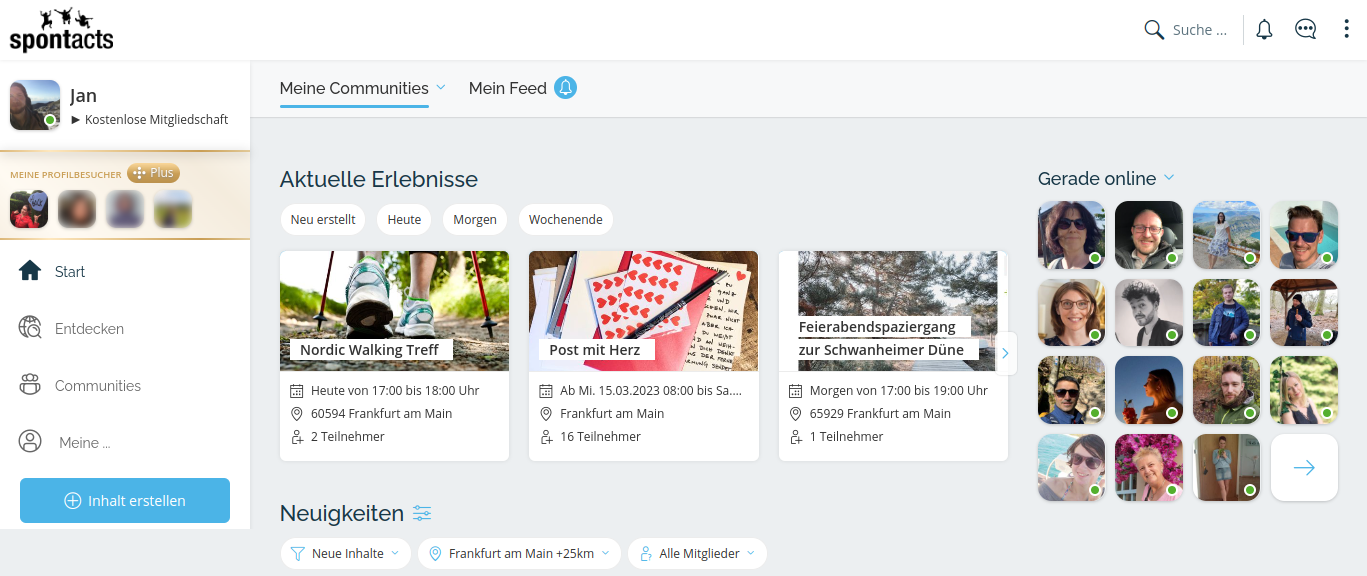
\includegraphics[width=\textwidth]{figures/jan/pic_spontacts.png}
    \caption[Startseite von Spontacts]{Startseite von Spontacts}
    \label{fig:spontacts}
\end{figure}

\paragraph{Selbstdarstellung}

Das Nutzerprofil auf Spontacts ähnelt dem anderer vergleichbarer Anwendungen und beinhaltet grundlegende Informationen wie den Namen, ein Profilbild, das Alter und den Wohnort. Es können jedoch auch weitere Angaben wie präferierte Kontakte für \textit{Freizeit}, \textit{Sport}, \textit{Reisen}, \textit{Tanzen} und \textit{Dating} oder zusätzliche Profilabschnitte (Hobbies, Interessen/Vorlieben usw.) hinzugefügt werden. Ein weiterer Abschnitt zeigt vergangene und zukünftige Aktivitäten des Nutzers sowie dessen Gruppenmitgliedschaften an.

\paragraph{Formen des Austausches}

Zur Interaktion mit anderen Benutzern können Beiträge in Spontacts erstellt werden. Diese Beiträge können je nach Art als einfacher Beitrag, als Aktivität oder als Frage/Diskussion verfasst werden und werden dann in Communities, Gruppen oder gegebenenfalls in Foren angezeigt. Wie gewohnt können sie kommentiert, gelikt und geteilt werden.

Die Communities sind eine Art Oberkategorie, die einen bestimmten Themenbereich (\textit{Ausgehen \&\ Party}, \textit{Essen \&\ Trinken}, \textit{Natur \&\ Umwelt} usw.) beschreiben und jedem Beitrag zugeordnet werden. Beim Erstellen einer Gruppe muss daher immer eine passende Community ausgewählt werden. Im Gegensatz zu den anderen vorgestellten Diensten sind Gruppen bei Spontacts das zentrale Feature der Anwendung. Sie ähneln in ihrem Funktionsumfang den Gruppen auf \acrshort{fb}.

Über die Beiträge hinaus können die Nutzer auch über den Chat eine private Unterhaltung führen. In diesem Chat können ausschließlich Textnachrichten ausgetauscht werden.

\paragraph{Recherche}

Um Beiträge, Veranstaltungen, Gruppen, Mitglieder und mehr zu entdecken, bietet Spontacts eine Suchfunktion mit spezifischen Filteroptionen je nach dem gesuchten Typ. Der Nutzer kann neben den allgemeinen Einstellungen wie Suchbegriff, Umkreis und Erstelldatum auch objektspezifische Kriterien wie Veranstaltungsdatum, Alter und ähnliches hinzufügen, um die Suche zu verfeinern.

Mitglieder können in die Kontakt- oder Merkliste aufgenommen werden, wenn sie für den Nutzer von Interesse sind. Die Merkliste ist eine private Liste, in die jedes Mitglied aufgenommen werden. Die Kontaktliste hingegen ist öffentlich und erfordert eine Bestätigung der Anfrage durch die betreffende Person. \\
Zusätzlich besteht die Möglichkeit, anderen Mitgliedern zu folgen, um ihre Aktivitäten besser verfolgen zu können. Wer wem folgt, kann in jedem Benutzerprofil eingesehen werden.

\paragraph{Neuigkeiten}

Um innerhalb der Plattform auf dem Laufenden zu bleiben, gibt es wie bei anderen Portalen ein Dashboard für Gruppen/Communities sowie einen Benachrichtigungs-Feed. Im Dashboard werden in der Rubrik \textit{Neuigkeiten} alle anstehenden Veranstaltungen und aktuellen Inhalte der Communities dargestellt. Unter der Rubrik \textit{Mein Feed} können hingegen alle Veränderungen in beigetretenen Gruppen eingesehen werden, wie beispielsweise neue Mitglieder und Veranstaltungen.\\
Der Benachrichtigungs-Feed enthält Informationen über neue Kontaktanfragen, Beiträge aus den Gruppen und Neuigkeiten über die Plattform.

\subsection{Strategische Ausrichtung}

Die drei Hauptwettbewerber weisen viele Gemeinsamkeiten auf, unterscheiden sich jedoch in ihrer strategischen Ausrichtung voneinander.

\acrshort{fb} ist eine sehr aktive Plattform, die sich darauf konzentriert, Menschen mit beliebigen Interessen, Themen und Bedürfnissen zu vernetzen, ohne dass der Nutzer dabei auf einen bestimmten geografischen Raum beschränkt ist. In letzter Zeit konnte keine intensive Weiterentwicklung der Plattform beobachtet werden, da sich das Unternehmen hauptsächlich der Entwicklung von zukünftigen Produkten im 3D-Umfeld widmet. Es ist daher lang- und mittelfristig keine Veränderung zu erwarten.

Nebenan.de ist der größte Konkurrent von \acrshort{dht}. Die Plattform ermöglicht es den Nutzern, sich in ihrer Nachbarschaft auszutauschen und zu vernetzen, wobei der Fokus auf der Stärkung der Gemeinschaft liegt. Eine große Herausforderung für Nebenan.de besteht darin, eine lebendige Community aufzubauen, die alle gesellschaftlichen Schichten und Altersklassen ansprechen.

Im Gegensatz dazu konzentriert sich Spontacts stark darauf, Menschen im privaten Bereich für gemeinsame Aktivitäten zu vernetzen. Die Plattform hat eine aktive Community, in der Nutzer Inhalte erstellen und an allen Veranstaltungen teilnehmen können, ohne harte lokale Einschränkungen wie bei nebenan.de. Darüber hinaus werden die Inhalte der Seite von lokal ansässigen Moderatoren betreut, die zusätzliche Veranstaltungen organisieren und durchführen. Strategisch setzt Spontacts zunehmend auf kostenpflichtige Accounts, die den Nutzern zusätzliche Funktionen wie verbesserte Filterfunktionen bieten sollen.

\subsection{Zusammenfassung}

Nach der Analyse der Konkurrenz wurde deutlich, dass die untersuchten Dienste ähnliche Funktionen wie Profile, Gruppen und Chats bereitstellen. Die Unterschiede zwischen den Features liegen eher in Nuancen, die von den jeweiligen Betreibern individuell gestaltet werden. \\
Die Plattformen unterscheiden sich jedoch in Bezug auf ihre Motivationen, Zielgruppen und geografischen Nutzerbereiche stark voneinander. Während einige Plattformen sich auf bestimmte Nachbarschaften beschränken, decken andere globale Communities ab. \\
Im Gegensatz dazu konzentriert sich \acrshort{dht} gezielt auf die Region/Gemeinde. Dadurch füllt \acrshort{dht} die Lücke zwischen \acrshort{fb} als weltweitem Akteur und nebenan.de mit Fokus auf die Nachbarschaft.

Ein weiterer Aspekt, der sich bei einem direkten Vergleich deutlich zeigt, ist die unterschiedliche Benutzerfreundlichkeit und Nutzerführung auf den verschiedenen Plattformen. Teils sind Inhalte schwer auffindbar und die zugrunde liegenden Konzepte sind nicht immer selbsterklärend. Um sicherzustellen, dass \acrshort{dht} für alle Altersgruppen verständlich ist, ist es unerlässlich, eine Plattform zu entwickeln, die einfach strukturiert und intuitiv zu bedienen ist.

Die Analyse zeigt anhand von nebenan.de und Spontacts, dass der Aufbau und die Etablierung eines sozialen Netzwerks viele Herausforderungen mit sich bringen. Als Vorreiter hat sich \acrshort{fb} in der Gesellschaft bereits stark etabliert und bietet mit einer breiten Palette von Features vielseitige Nutzungsmöglichkeiten für unterschiedliche Bedürfnisse. \\
Insbesondere für neue Plattformen stellt der Aufbau einer Community eine große Herausforderung dar. Als Newcomer müssen sie ohne bereits vorhandene Community und Content meist mit ähnlichen Funktionen wie Facebook die Nutzer überzeugen, dass ihre Plattform einen spürbaren Mehrwert im Vergleich zu Facebook bietet.
Gerade bei Plattformen, bei denen die Nutzer ausschließlich die Inhalte erstellen, gestaltet sich der Aufbau einer Community als besonders zäh, da neue Nutzer aufgrund mangelnder Inhalte schnell wieder abwandern können.\\
Daher ist es essentiell, dass kontinuierlich neue Inhalte zur Verfügung stehen, um sich zu etablieren. Spontacts setzt hierfür gezielt Moderatoren ein, um seinen Nutzern regelmäßig Angebote zu präsentieren. Alternativ kann die Bindung an ein Portal auch durch Angebote von Dritten erfolgen, wie zum Beispiel durch regelmäßige Informationen von Vereinen, Stadtverwaltungen oder Zeitungen, wie es bei \acrshort{dht} geplant ist. Zusätzliche Funktionen, wie ein Buchungsportal, können den Nutzern auch bei bestimmten Aktivitäten unterstützen.